
\documentclass[11pt]{article}

\usepackage[T1]{fontenc}
\usepackage[a4paper, top=1in, bottom=1.1in, left=1in, right=1in]{geometry}
\usepackage[toc,page]{appendix}
\usepackage[utf8]{inputenc} % utf8
\usepackage{amsmath}
\usepackage{attachfile}
\usepackage{booktabs}
\usepackage{caption}
\usepackage{commath}
\usepackage{graphicx}
\usepackage{hyperref}
\usepackage{listings}
\usepackage{mathtools}
\usepackage{siunitx}
\usepackage{subcaption}
\usepackage{tabularx}
\usepackage{url}
\usepackage{varioref}
\usepackage{wrapfig}
\usepackage{xcolor}

\setlength{\belowcaptionskip}{-6pt}
\makeatletter
\lst@Key{matchrangestart}{f}{\lstKV@SetIf{#1}\lst@ifmatchrangestart}
\def\lst@SkipToFirst{%
  \lst@ifmatchrangestart\c@lstnumber=\numexpr-1+\lst@firstline\fi
  \ifnum \lst@lineno<\lst@firstline
  \def\lst@next{\lst@BeginDropInput\lst@Pmode
    \lst@Let{13}\lst@MSkipToFirst
    \lst@Let{10}\lst@MSkipToFirst}%
  \expandafter\lst@next
  \else
  \expandafter\lst@BOLGobble
  \fi}
\makeatother

\lstset{  
  backgroundcolor=\color{gray!30},   % choose the background color; you must add \usepackage{color} or \usepackage{xcolor}
  basicstyle=\scriptsize,        % the size of the fonts that are used for the code
  breakatwhitespace=false,         % sets if automatic breaks should only happen at whitespace
  breaklines=true,                 % sets automatic line breaking
  captionpos=t,                    % sets the caption-position to bottom
  escapeinside={\%*}{*)},          % if you want to add LaTeX within your code
  extendedchars=true,              % lets you use non-ASCII characters; for 8-bits encodings only, does not work with UTF-8
  frame=single,                   % adds a frame around the code
  keepspaces=true,                 % keeps spaces in text, useful for keeping indentation of code (possibly needs columns=flexible)
  keywordstyle=\color{blue},       % keyword style
  language=C++,                 % the language of the code
  numbers=left,                    % where to put the line-numbers; possible values are (none, left, right)
  numbersep=20pt,                   % how far the line-numbers are from the code
  numberstyle=\tiny\color{gray}, % the style that is used for the line-numbers
  rulecolor=\color{blue!20},       
  showspaces=false,                % show spaces everywhere adding particular underscores; it overrides 'showstringspaces'
  showstringspaces=false,          % underline spaces within strings only
  showtabs=false,                  % show tabs within strings adding particular underscores
  stepnumber=1,                    % the step between two line-numbers. If it's 1, each line will be numbered
  tabsize=2,                   % sets default tabsize to 2 spaces
  framesep=7pt,
  xleftmargin=12pt,
  xrightmargin=11pt
}


\setlength{\fboxsep}{4pt}
\DeclareCaptionFormat{myformat}{%
  \hspace{1pt}\fcolorbox{blue!20}{gray!20}{\footnotesize\parbox{\dimexpr\textwidth-17pt\relax}{#1#2\ttfamily#3}}\vspace{-4pt}
}
\captionsetup[lstlisting]{format=myformat}

\captionsetup[figure]{labelfont=sf,hypcap=false,format=hang,margin=0.5cm,justification=RaggedRight,calcwidth=0.7\linewidth,font=footnotesize,justification=justified}
\captionsetup[subfigure]{labelfont=sf,hypcap=false,format=hang,margin=0.5cm,justification=RaggedRight,calcwidth=0.7\linewidth,font=footnotesize,justification=justified}
\captionsetup[table]{labelfont=sf,hypcap=false,format=hang,margin=1cm,justification=RaggedRight,calcwidth=0.8\linewidth,font=footnotesize,justification=justified}
\labelformat{equation}{(#1)}

%%% Math typesetting macros
\newcommand{\di}[2]{#1_\textup{#2}} % Descriptive Index: Macro for quick upright index (as opposed to a variable index, which should be italic)


\renewcommand{\lstlistlistingname}{Code listings}
\bibliographystyle{ieeetr}


%%%%%%%%%%%%%%%%%%%%%%%%%%%%%%
%%% STOLEN FROM STACKOVERFLOW
%%%%%%%%%%%%%%%%%%%%%%%%%%%%%%

\newcommand\YAMLcolonstyle{\color{red}\mdseries\scriptsize}
\newcommand\YAMLkeystyle{\color{black}\bfseries\scriptsize}
\newcommand\YAMLvaluestyle{\color{blue}\mdseries\scriptsize}

\makeatletter

% here is a macro expanding to the name of the language
% (handy if you decide to change it further down the road)
\newcommand\language@yaml{yaml}

\expandafter\expandafter\expandafter\lstdefinelanguage
\expandafter{\language@yaml}
{
  keywords={true,false,null,y,n},
  keywordstyle=\color{darkgray}\bfseries,
  basicstyle=\YAMLkeystyle,                                 % assuming a key comes first
  sensitive=false,
  comment=[l]{\#},
  morecomment=[s]{/*}{*/},
  commentstyle=\color{purple}\ttfamily,
  stringstyle=\YAMLvaluestyle\ttfamily,
  moredelim=[l][\color{orange}]{\&},
  moredelim=[l][\color{magenta}]{*},
  moredelim=**[il][\YAMLcolonstyle{:}\YAMLvaluestyle]{:},   % switch to value style at :
  morestring=[b]',
  morestring=[b]'',
  literate =    {---}{{\ProcessThreeDashes}}3
  {>}{{\textcolor{red}\textgreater}}1
  {|}{{\textcolor{red}\textbar}}1
  {\ -\ }{{\mdseries\ -\ }}3,
}

% switch to key style at EOL
\lst@AddToHook{EveryLine}{\ifx\lst@language\language@yaml\YAMLkeystyle\fi}
\makeatother

\newcommand\ProcessThreeDashes{\llap{\color{cyan}\mdseries-{-}-}}


\renewcommand{\tabularxcolumn}[1]{>{\small}m{#1}}
%%% Local Variables:
%%% mode: latex
%%% TeX-master: t
%%% End:

\bibliographystyle{ieeetr}
%% For make-title
\title{Laboration 3: Differential Drive with WiFi control\\ {\small Sensors and
    Sensing}} \author{Benny Frost, Tom Olsson} \date{\today}

\begin{document}
\maketitle %Title area
\begin{center}
  \emph{All code for this project can be found at \\
    \url{https://github.com/tgolsson/ros-arduino-wifi}}
\end{center}
\tableofcontents
\lstlistoflistings % List of all code snippets
\listoffigures % List of all figures
\listoftables \lstset{
  matchrangestart=t} %initialise the linerange-macro for \lstinput...


\section{Motivation and theory}
The goal of this project was to implement a differential drive robot based on
the Robot Operation System [ROS] on Arduino, which can be controlled using a
WiFi connection. While a differential drive is easy to implement and test using
a wired connection, most realistic scenarios will require wireless operation. As
ROS is very common in the scientific community, and Arduino is a cheap
prototyping platform in comparison to commercial robots, this could allow a
larger freedom in robot design. \par

The goals are:
\begin{itemize}
\item[$\Rightarrow$] To construct a robot with two powered wheels
\item[$\Rightarrow$] Setup the two motors with a differential drive controller
\item[$\Rightarrow$] Implement WiFi communication between PC and Arduino
\item[$\Rightarrow$] Tune the odometry
\end{itemize}

\subsection{PID with feedback}
PID in the name PID-controller is short for
\emph{Proportional}-\emph{Integral}-\emph{Derivative}-controller. As this
implies, the controlling signal is based on a proportion of the current error,
the previous error, and the rate of change of the observed error. Sometimes, the
error is augmented to include a part of the previous output value. In the case
of velocity control it can be used to counteract overshoot if the observable
value does not react instantly to output value. The mathematical formulation of
this is shown in \ref{eq:et}-\vref*{eq:pid}.\par \vspace{10pt} {\footnotesize
  \begin{tabular}{l l l}
    \textbf{Let:} \\
 &$e(t)$ &be some error measurement between current state x(t) and preferred state r(t)\\
 &$\di{K}{p}$, $\di{K}{i}$, $\di{K}{d}$ &be the respective weights for the proportional, integral and derivative terms \\
 &$u(t)$ &be the output signal at time \emph{t} \\
    \textbf{Then:}
  \end{tabular}
  \begin{align}
    e(t) &= r(t) - x(t) - u(t-1)\label{eq:et}\\
    u(t) &= \di{K}{p}\cdot e(t) + \di{K}{i} \cdot\int_{0}^{t}e(\tau)\cdot \dif\tau + \di{K}{d} \cdot \od{e(t)}{t}\label{eq:pid}
  \end{align}}
\par

This formulation of the PID controller borrows from feed-forward open-loop
control by partially ignoring the current measurements\footnote{An open loop
  controller has no sensory information: it has only state and model.}. The
controller is shown in fig. \vref{fig:pid}. \par
\begin{figure}[htb]
  \centering
  \begin{tikzpicture}[auto, node distance=2cm,>=latex']
    \node [input, name=rinput] (rinput) {}; \node [sum, right of=rinput, node
    distance=2cm] (sum1) {$\sum$}; \node [input, name=input2, above of=sum1]
    (input2) {}; \node [block, right of=sum1, node distance=4cm] (ki)
    {$\di{K}{I} \cdot \int_0^t e(t) $}; \node [block, above of=ki,node
    distance=1.5cm] (kp){$\di{K}{P}\cdot e(t)$}; \node [block, below of=ki,node
    distance=1.5cm] (kd) {$\di{K}{D} \cdot \frac{e(t)}{\dif t}$}; \node [sum,
    right of=ki,node distance=3cm] (sum2) {$\sum$}; \node [output, right
    of=sum2, node distance=2cm] (output) {}; \node [tmp, below of=kd,node
    distance=1cm] (tmp1){$\di{K}{F} \cdot u(t-1)$}; \draw [->] (rinput) --
    node{$r(t)$} (sum1); \draw [->] (input2) -- node{$x(t)$} (sum1); \draw [->]
    (sum1.east) -- node[midway,stacked,name=cen]{$e(t)$} (ki.west); \draw [->]
    (cen) |- (kp.west); \draw [->] (cen) |- (kd.west); \draw [->] (ki.east) --
    (sum2.west); \draw [->] (kp.east) -| (sum2.north); \draw [->] (kd.east) -|
    (sum2.south); \draw [->] (sum2) -- node[name=z]{$u(t)$} (output); \draw[->]
    (z) |- (tmp1); \draw[->] (tmp1) -| (sum1);
  

    \node [tmp, above left=0.05cm and -0.35cm of sum1] (abc1) {$-$}; \node [tmp,
    below left=0.05cm and -0.35cm of sum1] (abc2) {$-$}; \node [tmp, above
    left=-0.35cm and 0.05cm of sum1] (abc3) {$+$};
  
    \node [tmp, above left=0.05cm and -0.35cm of sum2] (abc4) {$+$}; \node [tmp,
    below left=0.05cm and -0.35cm of sum2] (abc5) {$+$}; \node [tmp, above
    left=-0.35cm and 0.05cm of sum2] (abc6) {$+$};

    \node [tmp, below of=tmp1,node distance=0.5cm] (abc7) {\tiny $u(t-1)$
      remapped to same range as $x(t)$ and $r(t)$};

  \end{tikzpicture}
  \caption[PID controller with feedback]{PID controller with feedback term.}
  \label{fig:pid}
\end{figure}\par

Another modification of PID controllers to improve motor control is the addition
of an output deadband or \emph{stiction}\footnote{A portmanteau of \emph{static
    friction}}. Stiction is the static cohesion threshold that needs to be
overcome in order to bring an object from rest when in contact with other
objects. In the case of a motor, this can be seen as the minimum
\texttt{PWM}-value where the shaft starts turning consistently.


\subsection{Communication protocols}
\label{sec:protocol}
As the \texttt{Arduino ros\_lib} implementation is based on the premise of
serial communication, some things need to be taken into consideration. No matter
whether operating over the USB port or a direct \texttt{TX,RX} connection a
serial protocol is always synced, and has a more or less constant rate of
information, and has predictable packet sizes. \par

TCP/IP on the other hand - which is the wireless protocol for a sustained
server/client connection - is not synced, nor does it make any guarantee on any
communication speeds. The only guarantee is that the data will arrive at some
point, and that it will be possible to retrieve the packages in proper
order. Compared to serial it also makes no guarantee on packet size; and may
sometimes try to limit the number of packages sent by collating many small
packets into larger ones using f.ex. Nagle's algorithm. \par

This discrepancy means that one cannot rely on data arriving regularly, and must
make sure that the implementation can handle the problems that can occur. These
problems could be a message being broken up into multiple parts, or only
receiving half the message, a connection dropout, etc.

\subsection{Differential Drive}
A differential drive is a kinematic model for two individually controlled wheels
used to control both speed and rotation by altering the relative speed between
the wheels. The controller implemented here is an inverse kinematic model; i.e.,
the desired output is given and then the parameters for the controller are calculated to give these
output parameters. \par
{\footnotesize
  \begin{tabular}{l l l}
    \textbf{Let:} \\
 &$v, \omega$ & be the desired linear (\emph{m/s}) and angular velocities (\emph{rad/s})\\
 &$L$ &be the distance between the two wheels \\
 &$r$ &be the radius of the robots wheels \\
 &$k$ &be the number of encoder ticks per shaft rotation\\
    &$u_l, u_r$ &be the left and right encoder speeds \\
    \textbf{Then:}
  \end{tabular}
  \begin{align}
    u_l &=  \frac{2\pi r}{k} \cdot \begin{cases}
                    \hspace{5pt}\left(\frac{v}{\omega} - L \right) * \omega \hspace{5pt} & if \omega \neq 0\\
                    \hspace{5pt} v & otherwise
                  \end{cases} \vspace{5pt} \\
    u_r &=  \frac{2\pi r}{k} \cdot \begin{cases}
                    \hspace{5pt}\left(\frac{v}{\omega} + L \right) * \omega \hspace{5pt} & if \omega \neq 0\\
                    \hspace{5pt}v & otherwise
                  \end{cases} 
  \end{align}}

\subsection{Odometry\label{sec:odometrymath}}
The kinematic model for differential drives can be used to estimate the robots
current position relative to the starting position. The equations for updating
the robots position are shown in
eq. \ref{eq:position1}-\vref*{eq:position2}. \par
{\footnotesize
  \begin{tabular}{l l l}
    \textbf{Let:} \\
 &$L$ &be the distance between the two wheels \\
 &$r$ &be the radius of the robots wheels \\
 &$k$ &be the number of encoder ticks per shaft rotation\\
 &$\hat{u}_l, \hat{u}_r$ &be the smoothed left and right measured encoder speeds (\emph{ticks/second})\\
&$x$, $y$, $\theta$ &be the position and rotation of the robot in a 2D coordinate system\\
    \textbf{Then:}
  \end{tabular}
  \begin{align}
    l_{left} &= \frac{2\pi r}{k} \cdot \hat{u}_l\label{eq:position1}\\
    l_{right} &= \frac{2\pi r}{k} \cdot \hat{u}_r\\
    \Delta &= \frac{(l_{right} - l_{left})}{L}\\
    d &= \frac{l_{right} + l_{left}}{2}\\
    \Delta_x &= \begin{cases}
                    \hspace{5pt}d \cdot \cos\left(\frac{\Delta}{2}\right) & if \left|\Delta\right| < \epsilon\\
                    \hspace{5pt}\frac{d}{\Delta} \cdot \sin\left(\Delta\right) & otherwise
                  \end{cases} \vspace{5pt}  \\
    \Delta_y &= \begin{cases}
                    \hspace{5pt}d \cdot \sin\left(\frac{\Delta}{2}\right) & if \left|\Delta\right| < \epsilon\\
                    \hspace{5pt}\frac{d}{\Delta} \cdot \left(1-\cos\left(\Delta\right)\right) & otherwise
                  \end{cases} \vspace{5pt}\\
    x_t &= x_{t-1} + \Delta_x \cdot \cos\left(\theta_{t-1}\right) - \Delta_y \cdot \sin\left(\theta_{t-1}\right)\\
    y_t &= y_{t-1} + \Delta_y \cdot \sin\left(\theta_{t-1}\right) + \Delta_y \cdot \cos\left(\theta_{t-1}\right)\\
    \theta_t &= \theta_{t-1} + \Delta\hspace{10pt}\label{eq:position2}
  \end{align}}

\section{Implementation}
The purpose of this project was to build a robot with two drive wheels. This
robot shall use an Arduino Due controller board with a differential drive
controller for these wheels, and communicate to a master node using WiFi and
TCP/IP. Part of the project is also measuring and tuning the accuracy for the
robots odometry.\par


\subsection{Hardware and environment}
The project used an \emph{Arduino Due} microcontroller \cite{arduinodue}, with
the \emph{Arduino Motor Shield R3} \cite{motorshield}. These are programmed
using Serial-over-USB; with the dedicated IDE. The version of the IDE used is
1.6.5. The project also includes usage of the \emph{Robot Operating System}
[ROS], version \emph{Indigo Igloo}. All ROS packages were installed directly
from GitHub. Two WiFi modules were tested during the project, the official
\emph{WiFi Shield R3} \cite{wifishield} as well as the \emph{ESP8266}
\cite{ESP8266}. \par
The motors used are the \emph{Micro Motors RHE158 75:1 12V DC} \cite{motors}.

% Hardware + Softwares used
\subsection{Physical design}
The main body of the robot is built from aluminum plating and profiles to get a
robust robot. The circuit boards are attached to Plexiglas which then are
attached to the main body. This is done to get a good insulation from the main
body. The Plexiglas pieces are attached with Velcro so it will be easy to detach
them if necessary. At front the two motors with the driving wheels was mounted
and two passive wheels where mounted at the back of the robot. The passive
wheels do not swivel and there was a concern if this would work. Testing showed
that the two electrical motors were too weak to be able to turn the robot with
this setup. This is probably because the friction against the floor is too
high. A centered swivel wheel was therefore mounted at the rear of the
robot. The robot is shown in fig. \vref{fig:robot}. \par

\begin{figure}[ht]
  \centering
  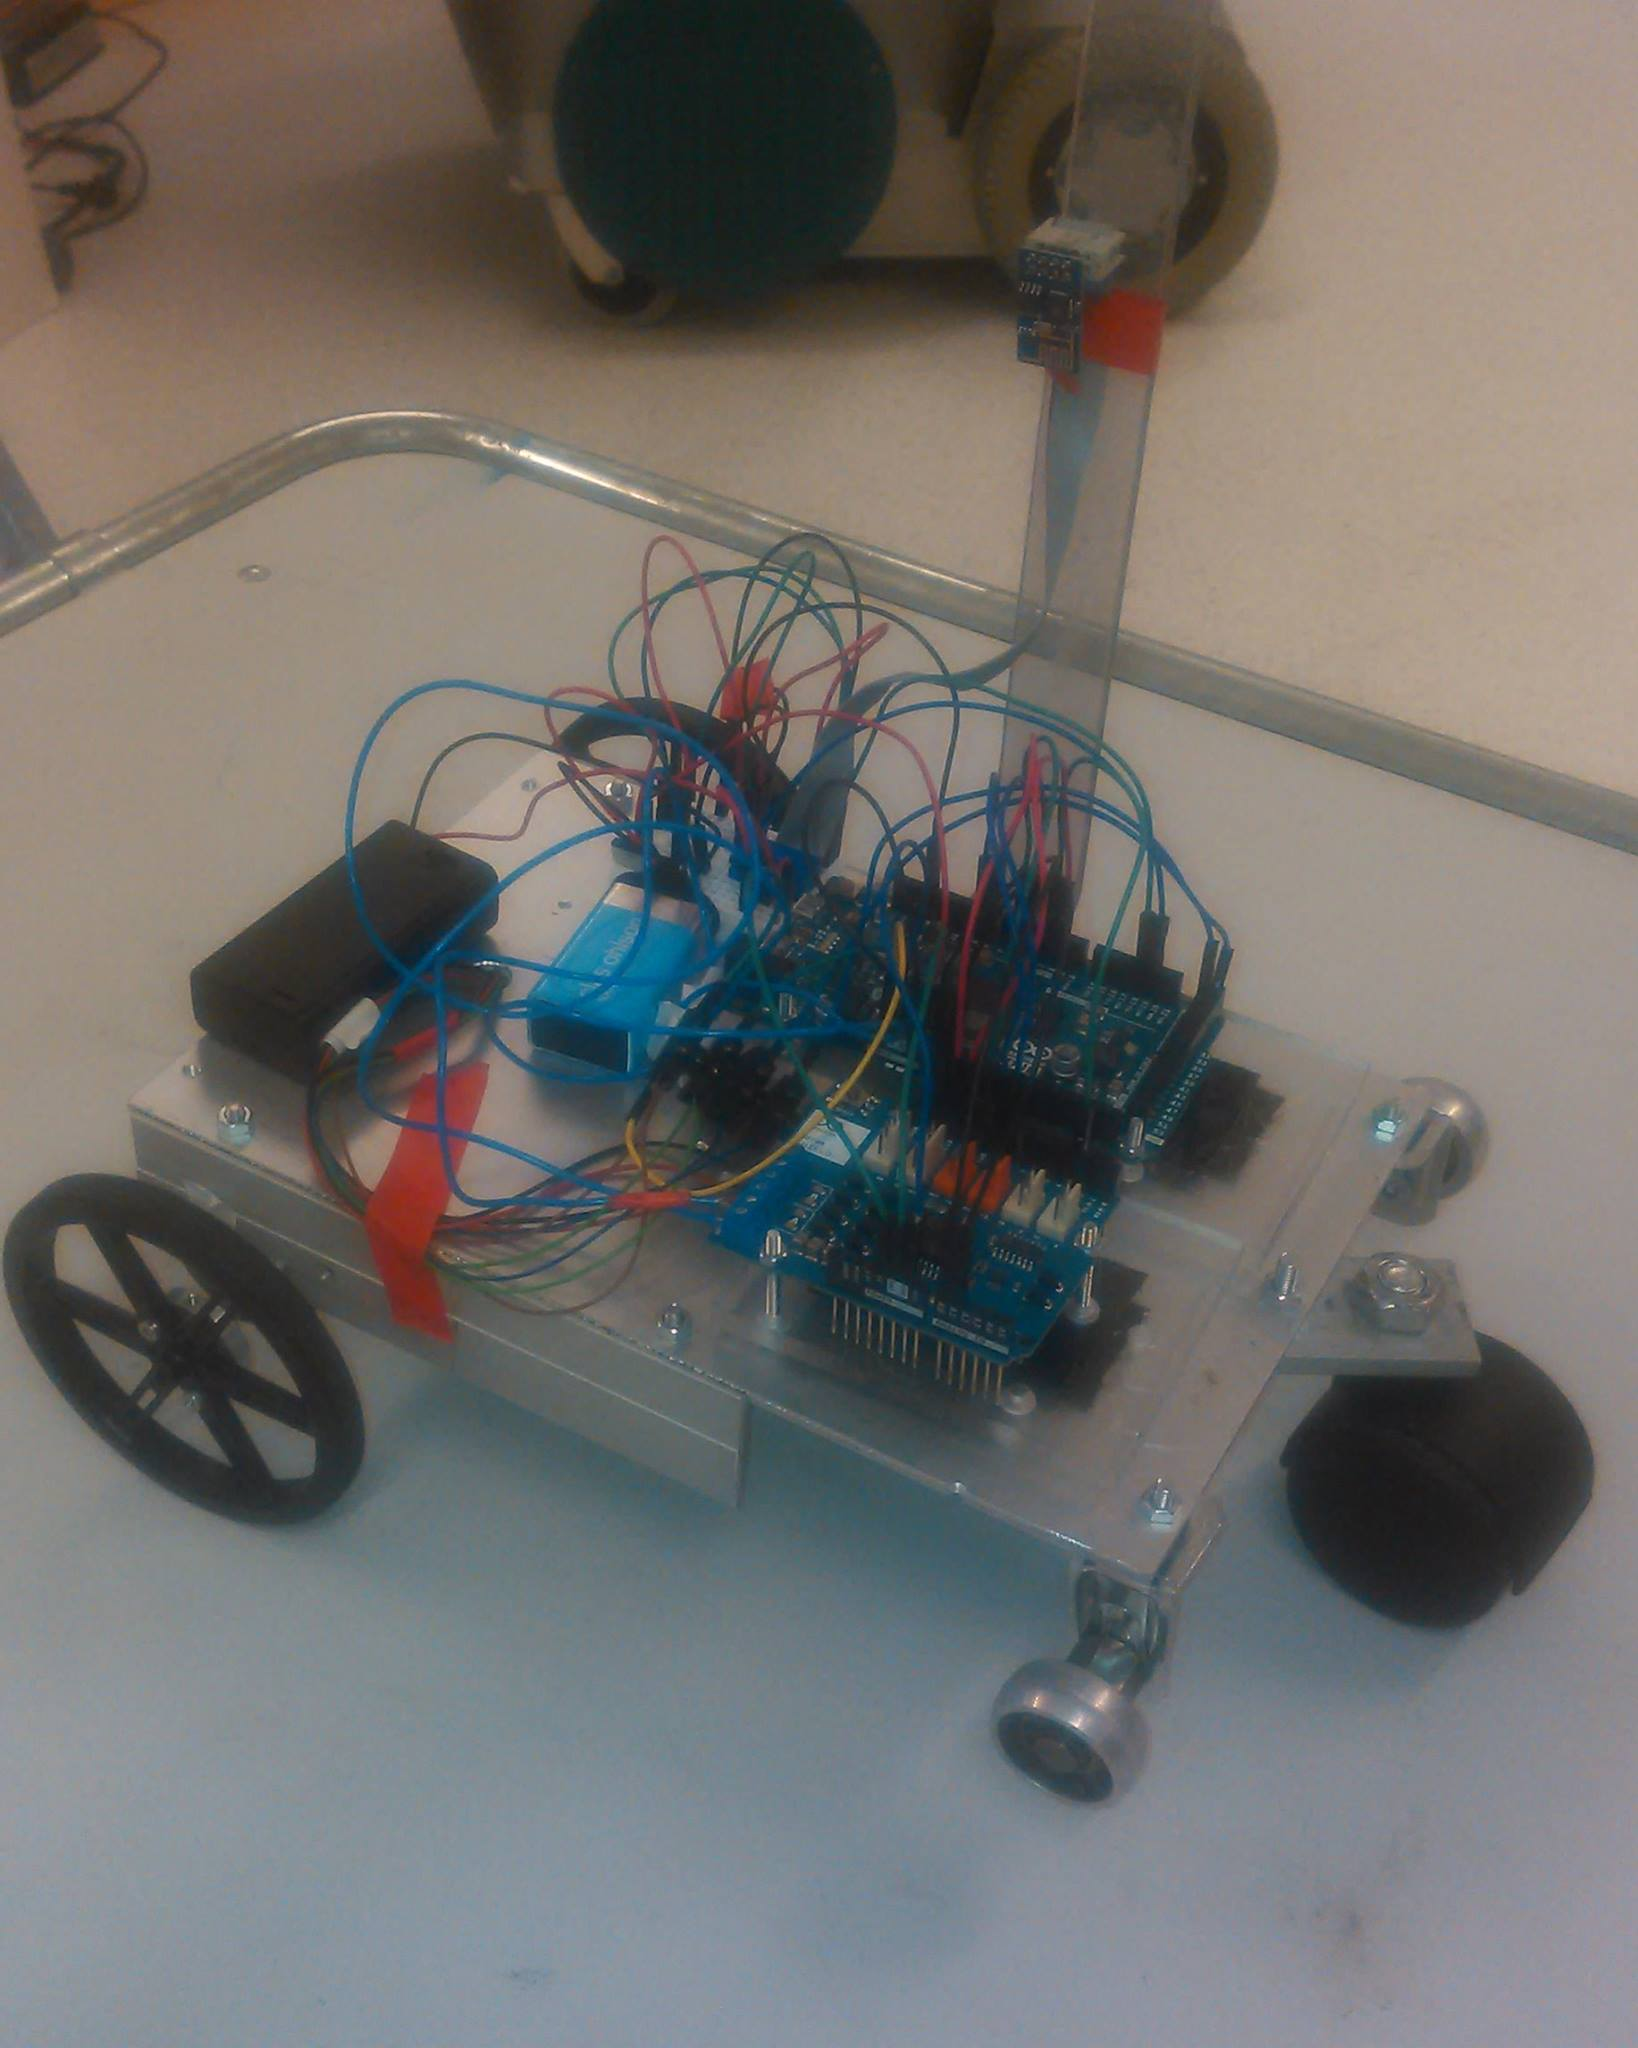
\includegraphics[width=.6\textwidth]{figures/robot.jpg}
  \captionof{figure}[Physical design of the robot]{\label{fig:robot} Physical
    design of the robot. The centered swivel wheel is at the back of the
    robot. Motor battery pack not mounted for better viewing.}
\end{figure}


For controlling the robot, an Arduino Due microcontroller is used with an
Arduino Motor Shield, and for communication an Arduino WiFi shield is
used. These two shields are made to sit on top of the Arduino Due. However, this
means that the WiFi shield and Motor shield will also sit on top of each
other. Since the WiFi shield and the Motor shield use the same I/O pins of the
Arduino Due it was decided that only the WiFi shield should be mounted on top of
the Arduino Due and the Motor shield should be mounted next to the main board
and be connected to the Arduino Due with wires, and by doing this I/O pins could
be rerouted to be used for the Motor shield. The WiFi shield was eventually
replaced with an EP8266 as described in the next section. Fig. \vref{fig:wiring}
shows how the Arduino Due, Arduino Motor shield and ESP8266 are connected. \par

\begin{figure}[ht]
  \centering
  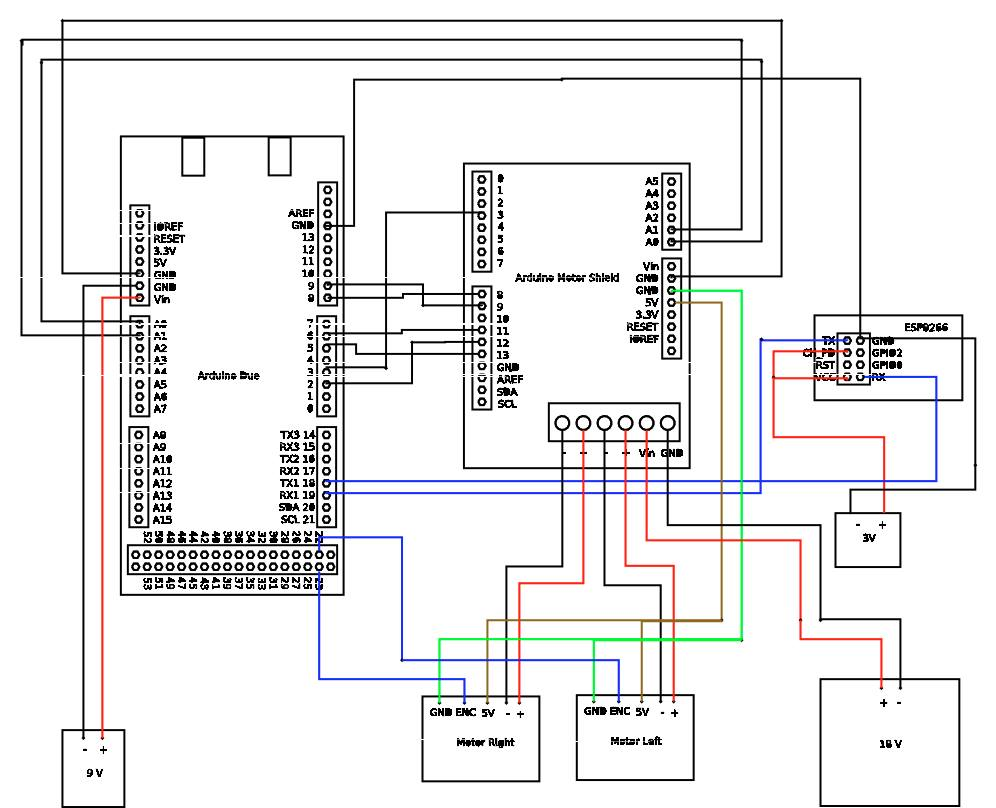
\includegraphics[width=.75\textwidth]{figures/wiring.jpg}
  \caption{\label{fig:wiring} The wiring diagram for the robot's electronics}
\end{figure}

\subsection{WiFi communication}
During setup and configuration of the Arduino WiFi shield it was obvious that
the communication was slow, taking almost two seconds from sending data to
reaching the destination, which was documented by others online
\cite{wificard1,wificard2}. Similarly, it was discovered that the largest
package that could be sent to the Arduino WiFi card is 92 bytes. If the package
is larger there will be a silent failure. Because of this it was decided to use
another WiFi card. We decided to use a popular combined microcontroller/WiFi
card, ESP8266. \par

The ESP8266 is a standalone microcontroller with built-in WiFi support
\cite{ESP8266}. This card is often recommended instead of the official WiFi card
both because of its cost as well as superior performance, which is the reason we
use it. Similarly to the normal Arduino boards it comes with its own toolchain,
and runs the code on its own in a separate process from the main Arduino
board. This allows the card to be setup to handle I/O asynchronously from the
main control loop which is a big performance gain. The final communication setup
is shown in fig. \vref{tikz:communicationschema}.\par

	\begin{figure}[h]
          \resizebox{1\linewidth}{!}{
            \begin{tikzpicture}[node distance=2cm]
              \begin{pgfonlayer}{main}
                \node (pc) [startstop] {PC (roscore)}; \node (serial) [process,
                below of=pc,yshift=-0.5cm, text width=4cm] {WiFi}; \node (esp)
                [startstop, right of=serial,xshift=3cm,text width=4.5cm]
                {ESP8266}; \node (deserialize) [process, right
                of=esp,xshift=3cm,text width=4cm] {UART}; \node (arduino)
                [startstop, above of=deserialize,yshift=0.5cm, text width=4cm]
                {Arduino};
				
                \draw [latex-latex,thick] (pc) -- (serial) node [midway, left]
                (TextNode) {}; \draw [latex-latex,thick] (serial) -- (esp) node
                [midway, left] (TextNode) {}; \draw [latex-latex,thick] (esp) --
                (deserialize) node [midway, left] (TextNode) {}; \draw
                [latex-latex,thick] (deserialize) -- (arduino) node [midway,
                left] (TextNode) {}; \draw [dashed,thick] (arduino.west) to[bend
                left=20] node[midway, above,yshift=0.5cm, anchor=center]
                (TextNode) {ROS communication} (pc.east);
              \end{pgfonlayer}
              \begin{pgfonlayer}{background}
                \node (kd) [draw=blue, fit=(pc) (serial) (esp), inner sep=0.15
                cm, inner ysep=0.5cm, yshift=-0.3cm, xshift=-1.375cm, inner
                xsep=-1cm, dashed, thick, fill=blue!10, fill opacity=0.2] {};
                \node [yshift=2ex, blue] at (kd.south) {TCP/IP communication};
				
                \node (kd) [draw=red, fit=(deserialize) (arduino) (esp), inner
                sep=0.15cm, inner ysep=0.5cm, yshift=-0.3cm, xshift=1.375cm,
                inner xsep=-1cm, dashed, thick, fill=red!10, fill opacity=0.2]
                {}; \node [yshift=2ex, red] at (kd.south) {Serial
                  communication};
              \end{pgfonlayer}
            \end{tikzpicture}
          }
          \captionof{figure}{System view of
            communication}\label{tikz:communicationschema}
	\end{figure}

        The PC and the Arduino both run \texttt{rosserial} to handle all
        communication and serialisation. To solve the issues raised in section
        \vref{sec:protocol} the baud rate between the ESP8266 and the Arduino
        Due was reduced by 33 \% compared to what \texttt{ros\_lib} uses normally
        at; to 38.4k from 57.6k. To further reduce the risk of dropping messages, the
        \texttt{NodeHandle} class was also modified to add a retry clause; where
        it would retry a second time whenever a message was at risk of being
        discarded. The code for this is shown in listing \vref{lst:retry}.

\newpage
\lstinputlisting[label=lst:retry,language=c++,caption={Code for error recovery
  in NodeHandle}, linerange={217-231
}]{/home/tgo/Arduino/libraries/ros_lib/ros/node_handle.h}

\subsection{Controller node}
The node used to steer the robot was developed by Husqvarna for their lawn mower
\emph{Auto Mower 320} and used for research at Örebro University. This node
fulfilled the requirements that was needed for this project. It is a Python
script that reads from the keyboard and publishes a
\texttt{geometry\_msgs::Twist} message on the ROS bus. The message uses
\texttt{linear.x} for forward speed and \texttt{angular.z} for angular speed.
\label{subsec:cn}


\subsection{Passthrough node}
\label{subsec:ptn}
The WiFi node is also simple. During startup it connects to a dedicated WiFi
router, and then connects to a hard-coded server IP. In the main \texttt{loop}
function it reads from the serial and writes to the WiFi; as well as from the
WiFi to the serial as was shown in fig. \vref{tikz:communicationschema}. To make
it more reliable the node checks both network and server connection each
iteration, and attempts to reconnect if any issues are detected. \par
The PC also runs the \texttt{roscore} as well as \texttt{rosserial\_python} in
TCP mode.
\subsection{Arduino node}
\label{subsec:dd}
This node has two PID controllers with their own $\di{K}{P}$, $\di{K}{I}$ and
$\di{K}{D}$ values, to set the velocity of the two wheels. It is necessary to
have two PID controllers since the motors appear to have slightly different
performance. \par

The PID controller uses the minimum jerk equation to control the setpoint value,
to ensure that the acceleration and deceleration is smooth. The implementation
used here is based on the derivation in \cite{mje} for estimating the rate of
change; and otherwise uses the canonical equation. \par

One major problem when implementing PID controllers to control the electrical
motors is the deadband of the motors. The value of the output from the PID
controller is clamped to [0,4095] and between 0-700 nothing happens. To solve
this; if the output is between 0-10 the output is set to 0, and if the output is
between 11-700 the output is set to 700, else the output is clamped to be in
between 700-4095.\par

The velocity of the motors is calculated by counting the number of interrupts
from the motors during one cycle of the controller. This input signal from the
encoders is then smoothed with a sliding window filter
(eq. \vref{eq:slidingwindow}), which means to get a velocity change to be fully
visible it takes around 330 ms with $\alpha=0.1$ and the controller running at
30 Hz. This also means there is a delay in the signal that the PID controller
receives, which skews the error value and by extension causes the controller to
overreact. As this mostly affects the integral term, it can cause the controller
to overshoot by a large margin. To counteract this, a fraction of the output is
fed back into the input as a promised velocity that will happen, so the
controller will not ramp up to high output and therefore not overshoot.\par

\begin{align}
  x_f(t) &= (1-\alpha) \cdot x_f(t-1)+  \alpha \cdot x(t)  \label{eq:slidingwindow}
\end{align}
For the communication with ESP8266 the Serial1 (\texttt{TX1,RX1}) is used
instead of the usual Serial/USB (\texttt{TX0,RX0}). With this setup it is still
possible to send debug data to the Arduino IDE with the USB connection.\par

The Arduino sketch uses \texttt{rosserial\_arduino} to handle all communication through the \texttt{NodeHandle}. The node subscribes to \texttt{/robot\_0/velocity\_commands}
(\texttt{geometry\_msgs::Twist}) to get the commands. It advertises its pose on
\texttt{/robot\_0/odometry} (\texttt{geometry\_msgs::Pose2D}). The Arduino
\texttt{loop} function runs at 30 Hz and the advertised topics are published
every third iteration.

\section{Results}
Overall the system performs well programmatically, with no bugs or crashes
inside the Arduino or the ESP8266. The device seems to run at a consistent
speed, and reacts quickly to new commands. There are some issues related to
network connectivity, with a dropped message once every two minutes on average,
as well as one recoverable connection loss in 30 minutes of runtime. However,
during execution these have no noticeable impact. \par

One major factor in network functionality seems to be the voltage of the ESP8266
battery pack. It is intended to operate with 3.3 V input voltage, and if it
drops down to 2.7-2.8 V it becomes significantly harder to connect and maintain
the connection. There is also a noticeable pulldown effect if the Arduino Due
battery pack drops in voltage, where the shared ground will pull down the
ESP8266 as well, therefore breaking the connection. Both the Arduino Due and the
ESP8266 seem to consume a lot of power as well; needing replacement batteries
after 40 minutes to an hour. Though 40 minutes is ample time for working inside
a lab, it imposes limits on practical usage of the robot; especially as
rechargeable batteries generally have lower energy density. \par

Lastly, there is significant work to be done on the design of the robot. Though
the robot works well in situations with few velocity changes, it suffers from
large inaccuracies during \emph{stop-go} scenarios. This is described in more
detail in section \vref{sec:odometry}.
\subsection{PID tuning}
\label{subsec:pidt}
The PID parameters were tuned by first setting up the $\di{K}{P}$ parameter to
achieve a good tracking when plotting the setpoint and the measured
velocity. When this tracking was smooth the $\di{K}{I}$ term was added until
overshoot appeared, and then both parameters were reduced in proportion until
overshoot stopped. This was required because of the smoothing applied to the
measured velocity. Once the behaviour was stable with different setpoints, the
$\di{K}{D}$ term was added to further reduce overshoot, as well as to stabilise
the value. \par

After adding and doing final tuning on the whole set of PID-values the feedback
term was added to the controller. The feedback term allowed us to reduce the
minimum-jerk rise-time while keeping overshoot low on large velocity changes. It
does so by acting as a promised velocity. Since the output of the PID - and by
extension the PWM value - maps directly to velocity, an output value is
instantly actuated as a change in speed. However due to the sliding window smoothing, only 10 \% of this change will
be visible in the next iteration, and then
19 \%, and so on. By feeding back the PWM value (converted to the internal
velocity measurement) we can reduce the error in proportion to our output PWM
value, which allows the error to closely track the real error without smoothing
applied. \par

Our final PID values are shown in table \vref{tab:pid}. These values are tuned
for movement on the ground with all battery packs on board. We found that the
PID values were different depending on whether the wheels were under load or
not. The values chosen provide a good trade-off between decent tracking,
reliable movement and quick reactions to commands. \par
\begin{center}
  
\begin{tabular}{r|c|l}
  Left motor & Parameter & Right motor \\
  23  & $\di{K}{P}$ & 24 \\
  36  & $\di{K}{I}$ & 35 \\
  0.1  & $\di{K}{D}$ & 0.1 \\
  0.05  & $Feedback$ & 0.05 
\end{tabular}
\captionof{table}[PID: Final parameters]{The final values used for the left
  respectively right motor controller. \label{tab:pid}}

\end{center}


\subsection{Odometry accuracy\label{sec:odometry}}
The position estimation of the robot (as described in section
\vref{sec:odometrymath}) is accurate given a few constraints, but inaccurate if
these are not met. During straight line or long smooth movements the robot has a
relative error of less than 1 \%. However when executing movements with multiple
changes in angular velocity the odometry does not keep up with the turning; and becomes
inaccurate. In this case, the errors can accumulate up to 3-4 \% of the distance
traveled. \par

One large part of this is the specific swivel wheel we use at the rear. When
starting with the wheel properly aligned with the direction of travel the errors
are small. However, after turning the wheel may be orthogonal to the vehicles
direction, and acts as a lever to twist the robot. However, this wheel is not
intended for usage in robots, and could therefore skew the results. The property
we believe influences the performance is the distance between the wheel
attachment rotation point, and the wheel friction point. In the case of our
wheel, this is almost as large as the wheel's radius. This means that to align
with the vehicles direction, the wheel needs to start rotating. During this
period of time, the wheel travels more easily in a direction orthogonal to the
vehicles movement, i.e., it rotates while at the same time applying friction in
the direction of travel causing slippage. \par

The effect described above primarily causes overturning, where a turning
movement continues for longer than intended while the swivel wheel corrects
itself. When using the original two static wheels however, the issues was the
opposite. In that case, the friction was orthogonal to the direction of travel
at all times, and therefore caused slippage during fast turning instead, causing
underturning. When testing the setup we found that a 90$^\circ$ turn could
result in as little as {30-45}$^\circ$ of actual turning, which is obviously
worse than the performance of the swivel wheel. \par

We measured the odometry with four different movement patterns. In all cases,
each movement action was discrete, i.e., each movement was fully completed
before the next one. As is common when measuring odometry we started by moving
in square patterns both counterclockwise (table \vref{tab:ccw}) and clockwise
(table \vref{tab:cw}). The square used was a 2x2 m in size, and counter-measured
along the diagonals to make sure it was perfectly square. The movement was
controlled using PC node, and the error in odometry was measured as the
difference between odometry position and actual position. As can be seen in
tables \ref{tab:ccw} and \ref{tab:cw} there is a high error during square
movements, especially when moving clockwise. The error is measured as absolute
value to make comparison easier, and to prevent opposite signs from skewing the
score. As can be seen there is also better performance when doing
counterclockwise turns instead of clockwise turns, though the sample is small in
this case. \par

\begin{center}
  \begin{tabular}{r|cc}
    Iteration & $|\text{Error}_x|$ [cm] & $|\text{Error}_y|$ [cm] \\ \hline
    1 & 26 & 0 \\
    2 & 28 & 3 \\
    3 & 36 & 6 \\ \hline
    Average & 30 & 3             
  \end{tabular}
  \captionof{table}[Odometry: Counterclockwise square]{Odometry accuracy during
    counterclockwise movement of a 2 m square.\label{tab:ccw}}
\end{center}\par

\begin{center}
  \begin{tabular}{r|cc}
    Iteration & $|\text{Error}_x|$ [cm] & $|\text{Error}_y|$ [cm] \\ \hline
    1 & 41 & 53 \\
    2 & 45 & 26 \\
    3 & 35 & 12 \\ \hline
    Average & 40 & 30         
  \end{tabular}
  \captionof{table}[Odometry: Clockwise square]{Odometry accuracy during
    clockwise movement of a 2 m square.\label{tab:cw}}\par
\end{center}
In order to prove the hypothesis that the number of turns has a correlation with
the actual performance we also measured the errors for a straight line as well
as with a single turn as shown in tables \ref{tab:straight} and
\vref{tab:singleturn}. As it was impossible to accurately measure the error in
$x$ and $y$ during the straight line while still moving a reasonable distance,
we calculated the hypotenuse of the position reported by the odometry and
compared this with the distance traveled in the real world. Obviously, if the
odometry is accurate these should be equal to each other. As can be seen in
table \ref{tab:straight} the error over almost four meters is less than 2
centimeters; compared to 40 centimeters over 8 meters in the case of the
clockwise square above. \par
To further prove this, we also measured the error when moving the full line and
coming back again; as this is the same method as with the square but with a
single \ang{180} rotation. As shown in table \ref{tab:singleturn} the error is
still small compared to above, though slightly bigger than in the case of no
turns. This, in addition to our visual observation of the robots movement and
the swivel wheel specifically shows that the error in measurements is directly
proportional to the number of direction changes in the path.
\begin{center}\begin{tabular}{r|ccc}
                Iteration & Measured [m] & Odometry [m] & |Error| [cm] \\ \hline
                1 & 3.84 & 3.81 & 2.97 \\
                2 & 3.52 & 3.51 & 0.64 \\
                3 & 3.47 & 3.45 & 1.96 \\
                4 & 3.96 & 3.94 & 1.79 \\
                5 & 3.95 & 3.93 & 1.84 \\ \hline
                Average & & & 1.84
              \end{tabular}
              \captionof{table}[Odometry: Straight line]{Odometry accuracy
                during straight line movement.\label{tab:straight}}\par
            \end{center}

            \begin{center}
              \begin{tabular}{r|cc}
                Iteration & $|\text{Error}_x|$ [cm] & $|\text{Error}_y|$ [cm] \\ \hline
                1 & 0 & 7 \\
                2 & 2 & 15 \\
                3 & 6 & 0 \\ \hline
                Average & 3 & 7
              \end{tabular}\par
              \captionof{table}[Odometry: two-way straight line]{Odometry
                accuracy during two-way movement along straight
                line.\label{tab:singleturn}}\par

            \end{center}

\newpage
\bibliography{references.bib}
\end{document}



%%% Local Variables:
%%% mode: latex
%%% TeX-master: t
%%% End:
